%
% Homework Details
%   - Title
%   - Due date
%   - University
%   - Class
%   - Class Alias
%   - Class Section
%   - Instructor
%   - Author
%   - AuthorID
%

\newcommand{\hmwkID}{3}
\newcommand{\hmwkTitle}{Homework\ \#\hmwkID}
\newcommand{\hmwkDueDate}{April 28, 2015 at 16:20}
\newcommand{\hmwkUniversity}{NTU}
\newcommand{\hmwkClass}{Data Structures and Algorithms}
\newcommand{\hmwkClassAlias}{DSA}
\newcommand{\hmwkClassSection}{Spring 2015}
\newcommand{\hmwkClassInstructor}{Hsuan-Tien Lin, Roger Jang}
\newcommand{\hmwkAuthorName}{Tim Liou}
\newcommand{\hmwkAuthorID}{b03902028}


\documentclass[11pt]{article}

\usepackage{fancyhdr}
\usepackage{extramarks}
\usepackage{enumitem}
\usepackage{amsmath}
\usepackage{amsthm}
\usepackage{amsfonts}
\usepackage{tikz}
\usepackage[plain]{algorithm}
\usepackage{algpseudocode}
\usepackage{listings}
\usepackage{lastpage}
\usepackage{color}

\usetikzlibrary{shapes,positioning,arrows,calc}
\usetikzlibrary{automata,positioning}

%
% Basic Document Settings
%

\topmargin=-0.45in
\evensidemargin=0in
\oddsidemargin=0in
\textwidth=6.5in
\textheight=9.0in
\headsep=0.25in

\linespread{1.1}

\pagestyle{fancy}
\lhead{\hmwkAuthorName\ (\hmwkAuthorID)}
\chead{\hmwkClassAlias\ (\hmwkUniversity, \hmwkClassSection): \hmwkTitle}
\rhead{\firstxmark}
\lfoot{\lastxmark}
\cfoot{\thepage\ of \pageref{LastPage}}

\renewcommand\headrulewidth{0.4pt}
\renewcommand\footrulewidth{0.4pt}

\setlength\parindent{0pt}
\setlength{\parskip}{1em}
%
% Create Problem Sections
%

\newcommand{\enterProblemHeader}[1]{
    \nobreak\extramarks{}{Problem \hmwkID.\arabic{#1} continued on next page\ldots}\nobreak{}
    \nobreak\extramarks{Problem \hmwkID.\arabic{#1} (continued)}{Problem \hmwkID.\arabic{#1} continued on next page\ldots}\nobreak{}
}

\newcommand{\exitProblemHeader}[1]{
    \nobreak\extramarks{Problem \hmwkID.\arabic{#1} (continued)}{Problem \hmwkID.\arabic{#1} continued on next page\ldots}\nobreak{}
    \stepcounter{#1}
    \nobreak\extramarks{Problem \hmwkID.\arabic{#1}}{}\nobreak{}
}

\setcounter{secnumdepth}{0}
\newcounter{partCounter}
\newcounter{homeworkProblemCounter}
\setcounter{homeworkProblemCounter}{1}
\nobreak\extramarks{Problem \hmwkID.\arabic{homeworkProblemCounter}}{}\nobreak{}

%
% Homework Problem Environment
%
% This environment takes an optional argument. When given, it will adjust the
% problem counter. This is useful for when the problems given for your
% assignment aren't sequential. See the last 3 problems of this template for an
% example.
%
\newenvironment{homeworkProblem}[2][-1]{
    \ifnum#1>0
        \setcounter{homeworkProblemCounter}{#1}
    \fi
    \section{\hmwkID.\arabic{homeworkProblemCounter} \hspace{0.1in} #2}
    \setcounter{partCounter}{1}
    \enterProblemHeader{homeworkProblemCounter}
}{
    \exitProblemHeader{homeworkProblemCounter}
}

%
% Title Page
%

\title{
    \vspace{2in}
    \textmd{\textbf{\hmwkClass:\ \hmwkTitle}}\\
    \normalsize\vspace{0.1in}\small{Due\ on\ \hmwkDueDate}\\
    \vspace{0.1in}\large{\textit{Instructors \hmwkClassInstructor}}
    \vspace{3in}
}

\author{
    \textbf{\hmwkAuthorName} \small{(\hmwkAuthorID)} 
}
\date{}

\renewcommand{\part}[1]{\textbf{\large Part \Alph{partCounter}}\stepcounter{partCounter}\\}

\lstset{
    language=C,
    numbers=left,
    frame=single,
    columns=fullflexible,
    basicstyle=\ttfamily
}

%
% Various Helper Commands
%

\newcommand{\subqest}[1]{ \textbf{(\arabic{partCounter})} #1 \stepcounter{partCounter} \par }

% Something need to be done
\newcommand{\pending}[1][]{~~~~\textcolor{red}{ 
        \textbf{ \large ====== Pending 
            \ifx&#1&%
            % #1 is empty
            \else
            % #1 is nonempty
            \large (#1)
            \fi
            \large ====== 
        } 
    }
}

% Useful for algorithms
\newcommand{\alg}[1]{\textsc{\bfseries \footnotesize #1}}

% For derivatives
\newcommand{\deriv}[1]{\frac{\mathrm{d}}{\mathrm{d}x} (#1)}

% For partial derivatives
\newcommand{\pderiv}[2]{\frac{\partial}{\partial #1} (#2)}

% Integral dx
\newcommand{\dx}{\mathrm{d}x}

% Alias for the Solution section header
\newcommand{\solution}{\textbf{\large Solution}}

% Probability commands: Expectation, Variance, Covariance, Bias
\newcommand{\E}{\mathrm{E}}
\newcommand{\Var}{\mathrm{Var}}
\newcommand{\Cov}{\mathrm{Cov}}
\newcommand{\Bias}{\mathrm{Bias}}




\begin{document}

\pagenumbering{gobble}

\maketitle

\pagebreak

\pagenumbering{arabic}  

\begin{homeworkProblem}{Asymptotic Complexity}
    \subqest{Do Exercise R-4.28 of the textbook.}
    Consider $a_k \geq 0~for~k \geq 0$
    \[
        \begin{split}
            p(n) = a_0 + a_1n + a_2n^2 + a_3n^3 + \dots + a_mn^m
        \end{split}
    \]

    For $n \geq (a_0 + a_1 + a_2 + \dots + a_m) \geq 1$, we have
    \[
        \begin{split}
            p(n) &\leq (a_0 + a_1 + a_2 + \dots + a_m) \times n^m
            \\
            \Rightarrow \log p(n) &\leq \log (a_0 + a_1 + a_2 + \dots + a_m) + m\log n
            \\
            &\leq \log n + m \log n
            \\
            &= (m+1) \log n
        \end{split}
    \]
    Take $c = m+1 > 0$, $n_0 = (a_0 + a_1 + a_2 + \dots + a_m) \geq 1$
    \[
        \begin{split}
            \log p(n) \leq c\log n~~for~n \geq n_0
        \end{split}
    \]
    That is, $\log p(n)$ is $O(\log n)$.


    \subqest{Do Exercise R-4.34 of the textbook.}
    We have $f(n) > 1$ and $\lceil f(n) \rceil \leq f(n) + 1$ by definition. For $n \geq 1$,
    \[
        \begin{split}
            \lceil f(n) \rceil &\leq f(n) + 1
            \\
            &\leq f(n) + f(n)
            \\
            &= 2f(n)
        \end{split}
    \]
    Take $c = 2 > 0$, $n_0 = 1 \geq 1$
    \[
        \begin{split}
            \lceil f(n) \rceil \leq cf(n)~~for~n \geq n_0
        \end{split}
    \]
    That is, $\lceil f(n) \rceil$ is $O(f(n))$.


    \subqest{Prove that $f(n) = \Theta(g(n))$.}
    By definition of limits at infinity,
    \[
        \begin{split}
            \lim_{n \to \infty} \frac{f(n)}{g(n)} = A
        \end{split}
    \]
    means that for every $\epsilon > 0$ there is a corresponding $N$ such that
    \[
        \begin{split}
            |\frac{f(n)}{g(n)} - A| < \epsilon ~~~for~n>N
        \end{split}
    \]

    That is,
    \[
        \begin{split}
            A - \epsilon < \frac{f(n)}{g(n)} < A + \epsilon ~~~for~n>N
        \end{split}
    \]

    Note that $g(n)$ is a strictly positive function. We have
    \[
        \begin{split}
            (A - \epsilon)g(n) < f(n) < (A + \epsilon)g(n) ~~~for~n>N
        \end{split}
    \]

    Take $\epsilon \in (0,A)$, $c_1 = (A - \epsilon) > 0$, $c_2 = (A + \epsilon) > 0$, $n_0 > N$
    \[
        \begin{split}
            c_1 g(n) \leq f(n) \leq c_2 g(n) ~~~for~n>n_0
        \end{split}
    \]
    This shows that $f(n) = \Theta(g(n))$.


    \subqest{Do Exercise R-4.8 of the textbook.}
    If A is better than B for $n \geq n_0$, $n_0$ satisfies the following statement.
    \[
        \begin{split}
            2{n_0}^3 - 40{n_0}^2 > 0
        \end{split}
    \]
    We can easily find that $n_0 > 20$. We choose $n_0 = 21$. It is a possible value for $n_0$ 
    satisfying the statement that A is better than B for $n \geq n_0$.
    
    
    \subqest{Do Exercise C-4.16(b) of the textbook.}
    This is the pseudo code of the Horner's method.
    \begin{algorithm}[]
        \begin{algorithmic}[1]
            \Function{Horner's-Method}{\emph{x,~CoefficientsOfPolynomial,~DegreeOfPolynomial}}
            \State{$Sum \gets 0$}
            \ForAll{\emph{CoefficientsOfPolynomial}}
                \State{$Sum \gets Sum \times x + \emph{CoefficientsOfPolynomial}$}
            \EndFor
            \State{\Return{$Sum$}}
            \EndFunction{}
        \end{algorithmic}
        \caption{Horner's method for computing polynomial}
    \end{algorithm}

    We can find there is only one \alg{for loop} in this pseudo code, that is, the number of 
    arithmetic operations is $O(n)$.


    \pagebreak

    \subqest{Consider some $f(n)$ and $g(n)$ such that $\lg f(n) = O(\lg g(n))$ and $g(n) \geq 2$
    for $n \geq 1$. Construct a counter-example to disprove that $f(n) = O(g(n))$.}
    Consider $f(n) = 4^n$, $g(n) = 2^n$, for $n \geq 1$, we can find
    \[
        \begin{split}
            \lg f(n) &= n 2 \lg 2 
            \\
            &\leq n 4\lg 2 
            \\
            &= 4 \lg 2^n
            \\
            &= 4\lg g(n)
        \end{split}
    \]

    Take $c = 4 > 0$, $n_0 = 1 \geq 1$
    \[
        \begin{split}
            \lg f(n) \leq c \lg g(n)~~for~n \geq n_0
        \end{split}
    \]
    That is, $\lg f(n)$ is $O(\lg g(n))$. Note that $g(n) \geq 2$ for $n \geq 1$.

    If $f(n) = O(g(n))$, $\exists n_0 > 0, c > 0 \ni$
    \[
        \begin{split}
            4^n \leq c 2^n~~for~n \geq n_0
        \end{split}
    \]
    Take $\log_2$ on both sides,
    \[
        \begin{split}
            &2n \leq \log_2 c + n~~for~n \geq n_0 \\
            &\Rightarrow \log_2 c \geq n
        \end{split}
    \]
    That is, take $n^{\prime} = max(n_0, \lceil \log_2 c + 1 \rceil)$
    \[
        \begin{split}
            n^{\prime} \geq n_0 &\Rightarrow 4^n \leq c 2^n \\
            n^{\prime} > \log_2 c &\Rightarrow 4^n > c 2^n \\
        \end{split}
    \]
    This is a contradiction. Therefore, we disprove that $f(n) = O(g(n))$.

\end{homeworkProblem}

\pagebreak

\begin{homeworkProblem}{Stack, Queue, Deque}

    \subqest{Do Exercise C-5.2 of the textbook.}
    Pop out the elements in the stack one by one and check if it is equal to element $x$. After that,
    enqueue the elements into the queue one by one. Use a varible to store the number of the 
    elements we poped from the stack. Once we find the certain element or the stack is empty, we push
    the elements into stack from queue, and then enqueue the same number of element into queue from
    stack. Finally push all these elements from queue into stack again. This will maintain elements'
    original order.

    \begin{figure}[h!]
        \centering
        \begin{tikzpicture}[stack/.style={
                rectangle split, rectangle split parts=9, draw, anchor=center},
            myarrow/.style={single arrow, draw=none}]

            \node [stack] (s0)  {
            \nodepart{three}$e_n$\nodepart{four}$\vdots$\nodepart{five}$x$
            \nodepart{six}$\vdots$\nodepart{seven}$e_2$\nodepart{eight}$e_1$
            \nodepart{nine}$e_0$};
            \node [stack,right=of s0] (q0) {\nodepart{five}$\vdots$};
            \node [above=of s0,anchor=north,align=left] {S};
            \node [above=of q0,anchor=north,align=left] {Q};

            \node [myarrow,draw,right=of q0] (a1) {\phantom{te}} ;

            \node [stack,right=of a1] (s1)  {
            \nodepart{six}$\vdots$\nodepart{seven}$e_2$\nodepart{eight}$e_1$
            \nodepart{nine}$e_0$};
            \node [stack,right=of s1] (q1) {
            \nodepart{five}$x$
            \nodepart{six}$\vdots$\nodepart{seven}$e_{n-2}$\nodepart{eight}$e_{n-1}$
            \nodepart{nine}$e_n$};
            \node [above=of s1,anchor=north,align=left] {S};
            \node [above=of q1,anchor=north,align=left] {Q};

            \node [myarrow,draw,right=of q1] (a2) {\phantom{te}} ;

            \node [stack,right=of a2] (s2)  {
            \nodepart{three}$x$\nodepart{four}$\vdots$\nodepart{five}$e_n$
            \nodepart{six}$\vdots$\nodepart{seven}$e_2$\nodepart{eight}$e_1$
            \nodepart{nine}$e_0$};
            \node [stack,right=of s2] (q2) {\nodepart{five}$\vdots$};
            \node [above=of s2,anchor=north,align=left] {S};
            \node [above=of q2,anchor=north,align=left] {Q};

            \node [myarrow,draw,anchor=north] (a3) at ($(a1.south)+(0,-190pt)$) {\phantom{te}} ;

            \node [stack,right=of a3] (s3)  {
            \nodepart{six}$\vdots$\nodepart{seven}$e_2$\nodepart{eight}$e_1$
            \nodepart{nine}$e_0$};
            \node [stack,right=of s3] (q3) {
            \nodepart{nine}$x$
            \nodepart{eight}$\vdots$\nodepart{seven}$e_{n-2}$\nodepart{six}$e_{n-1}$
            \nodepart{five}$e_n$};
            \node [above=of s3,anchor=north,align=left] {S};
            \node [above=of q3,anchor=north,align=left] {Q};

            \node [myarrow,draw,right=of q3] (a4) {\phantom{te}} ;

            \node [stack,right=of a4] (s4)  {
            \nodepart{three}$e_n$\nodepart{four}$\vdots$\nodepart{five}$x$
            \nodepart{six}$\vdots$\nodepart{seven}$e_2$\nodepart{eight}$e_1$
            \nodepart{nine}$e_0$};
            \node [stack,right=of s4] (q4) {\nodepart{five}$\vdots$};
            \node [above=of s4,anchor=north,align=left] {S};
            \node [above=of q4,anchor=north,align=left] {Q};
        \end{tikzpicture}
        \caption{How this algorithm works}
    \end{figure}


    \pagebreak

    \subqest{Do Exercise C-5.9 of the textbook.}
    \begin{figure}[h!]
        \centering
        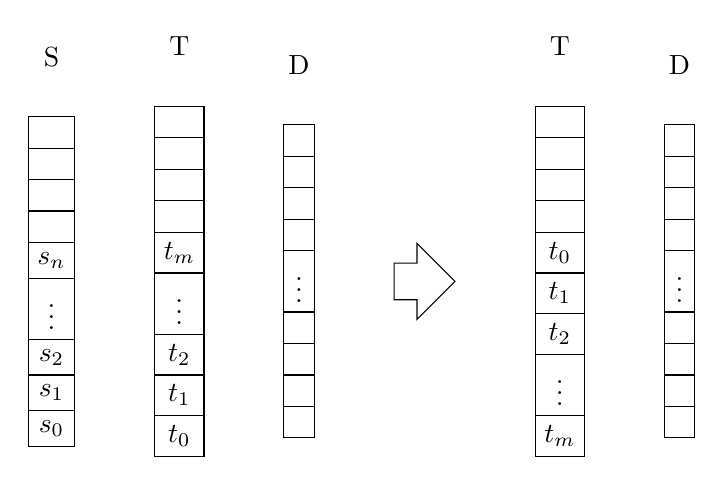
\begin{tikzpicture}[stack/.style={
                rectangle split, rectangle split parts=9, draw, anchor=center},
            myarrow/.style={single arrow, draw=none}]

            \node [stack] (s0)  {
            \nodepart{five}$s_n$
            \nodepart{six}$\vdots$\nodepart{seven}$s_2$\nodepart{eight}$s_1$
            \nodepart{nine}$s_0$};
            \node [stack,right=of s0] (t0) {
            \nodepart{five}$t_m$
            \nodepart{six}$\vdots$\nodepart{seven}$t_2$\nodepart{eight}$t_1$
            \nodepart{nine}$t_0$};
            \node [stack,right=of t0] (d0) {\nodepart{five}$\vdots$};
            \node [above=of s0,anchor=north,align=left] {S};
            \node [above=of t0,anchor=north,align=left] {T};
            \node [above=of d0,anchor=north,align=left] {D};

            \node [myarrow,draw,right=of d0] (a1) {\phantom{te}} ;

            \node [stack,right=of a1] (t1) {
            \nodepart{nine}$t_m$
            \nodepart{eight}$\vdots$\nodepart{seven}$t_2$\nodepart{six}$t_1$
            \nodepart{five}$t_0$};
            \node [stack,right=of t1] (d1) {\nodepart{five}$\vdots$};
            \node [above=of t1,anchor=north,align=left] {T};
            \node [above=of d1,anchor=north,align=left] {D};

        \end{tikzpicture}
        \caption{\alg{Pop} all elements from T and \alg{Push\_front} them to D. Then 
                 \alg{Pop\_back} them back to T.}
    \end{figure}

    \begin{figure}[h!]
        \centering
        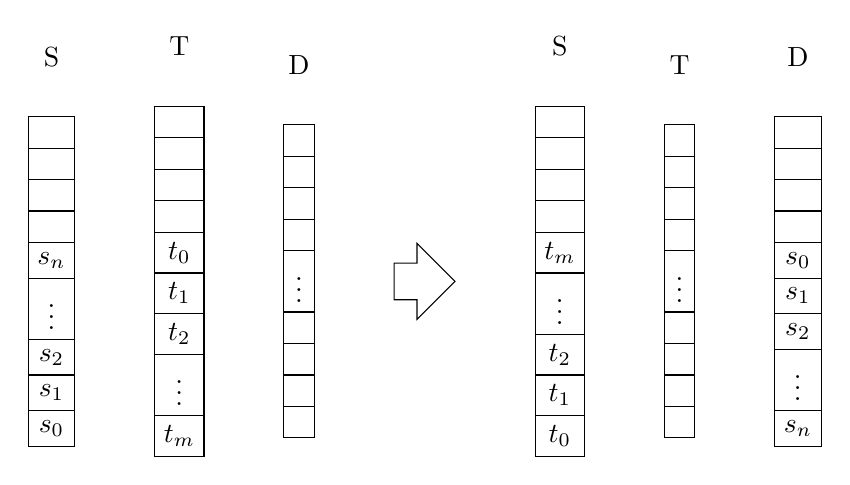
\begin{tikzpicture}[stack/.style={
                rectangle split, rectangle split parts=9, draw, anchor=center},
            myarrow/.style={single arrow, draw=none}]

            \node [stack] (s0)  {
            \nodepart{five}$s_n$
            \nodepart{six}$\vdots$\nodepart{seven}$s_2$\nodepart{eight}$s_1$
            \nodepart{nine}$s_0$};
            \node [stack,right=of s0] (t0) {
            \nodepart{nine}$t_m$
            \nodepart{eight}$\vdots$\nodepart{seven}$t_2$\nodepart{six}$t_1$
            \nodepart{five}$t_0$};
            \node [stack,right=of t0] (d0) {\nodepart{five}$\vdots$};
            \node [above=of s0,anchor=north,align=left] {S};
            \node [above=of t0,anchor=north,align=left] {T};
            \node [above=of d0,anchor=north,align=left] {D};

            \node [myarrow,draw,right=of d0] (a1) {\phantom{te}} ;

            \node [stack,right=of a1] (s1)  {
            \nodepart{five}$t_m$
            \nodepart{six}$\vdots$\nodepart{seven}$t_2$\nodepart{eight}$t_1$
            \nodepart{nine}$t_0$};
            \node [stack,right=of s1] (t1) {\nodepart{five}$\vdots$};
            \node [stack,right=of t1] (d1) {
            \nodepart{nine}$s_n$
            \nodepart{eight}$\vdots$\nodepart{seven}$s_2$\nodepart{six}$s_1$
            \nodepart{five}$s_0$};
            \node [above=of s1,anchor=north,align=left] {S};
            \node [above=of t1,anchor=north,align=left] {T};
            \node [above=of d1,anchor=north,align=left] {D};

        \end{tikzpicture}
        \caption{\alg{Pop} all elements from S and \alg{Push\_front} them to D. Then 
                 \alg{Pop} all elements from T to S.}
    \end{figure}

    \begin{figure}[h!]
        \centering
        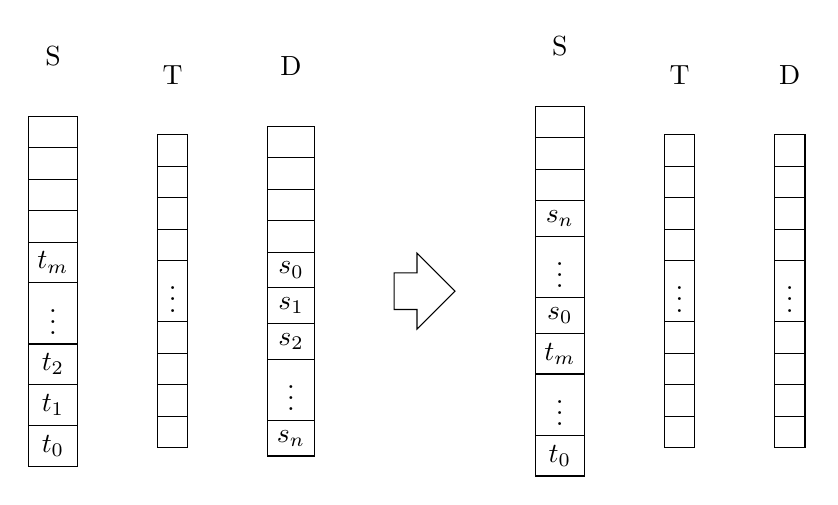
\begin{tikzpicture}[stack/.style={
                rectangle split, rectangle split parts=9, draw, anchor=center},
            myarrow/.style={single arrow, draw=none}]

            \node [stack] (s0)  {
            \nodepart{five}$t_m$
            \nodepart{six}$\vdots$\nodepart{seven}$t_2$\nodepart{eight}$t_1$
            \nodepart{nine}$t_0$};
            \node [stack,right=of s0] (t0) {\nodepart{five}$\vdots$};
            \node [stack,right=of t0] (d0) {
            \nodepart{nine}$s_n$
            \nodepart{eight}$\vdots$\nodepart{seven}$s_2$\nodepart{six}$s_1$
            \nodepart{five}$s_0$};

            \node [above=of s0,anchor=north,align=left] {S};
            \node [above=of t0,anchor=north,align=left] {T};
            \node [above=of d0,anchor=north,align=left] {D};

            \node [myarrow,draw,right=of d0] (a1) {\phantom{te}} ;

            \node [stack,right=of a1] (s1)  {
            \nodepart{four}$s_n$\nodepart{five}$\vdots$
            \nodepart{six}$s_0$\nodepart{seven}$t_m$
            \nodepart{eight}$\vdots$ \nodepart{nine}$t_0$};
            \node [stack,right=of s1] (t1) {\nodepart{five}$\vdots$};
            \node [stack,right=of t1] (d1) {\nodepart{five}$\vdots$};
            \node [above=of s1,anchor=north,align=left] {S};
            \node [above=of t1,anchor=north,align=left] {T};
            \node [above=of d1,anchor=north,align=left] {D};

        \end{tikzpicture}
        \caption{\alg{Pop\_front} all elements from D to S}
    \end{figure}


    \pagebreak

    \subqest{Use any pseudocode to write down an algorithm that uses two stacks 
    (with push, pop and isempty operations but no others) to simulate one deque
    (for push/pop front and push/pop back operations).
    What is the total running time after N operations?}
    \pending

    \subqest{Do Exercise C-5.9 of the textbook, but with three stacks instead of two stacks and 
    one deque.}
    Suppose three stacks are big enough for all elements.

    \begin{figure}[h!]
        \centering
        \begin{tikzpicture}[stack/.style={
                rectangle split, rectangle split parts=9, draw, anchor=center},
            myarrow/.style={single arrow, draw=none}]

            \node [stack] (s0)  {
            \nodepart{five}$s_n$
            \nodepart{six}$\vdots$\nodepart{seven}$s_2$\nodepart{eight}$s_1$
            \nodepart{nine}$s_0$};
            \node [stack,right=of s0] (t0) {
            \nodepart{five}$t_m$
            \nodepart{six}$\vdots$\nodepart{seven}$t_2$\nodepart{eight}$t_1$
            \nodepart{nine}$t_0$};
            \node [stack,right=of t0] (e0) {\nodepart{five}$\vdots$};
            \node [above=of s0,anchor=north,align=left] {S};
            \node [above=of t0,anchor=north,align=left] {T};
            \node [above=of e0,anchor=north,align=left] {E};

            \node [myarrow,draw,right=of d0] (a1) {\phantom{te}} ;

            \node [stack,right=of a1] (s1) {\nodepart{five}$\vdots$};
            \node [stack,right=of s1] (t1) {\nodepart{five}$\vdots$};
            \node [stack,right=of t1] (e1) {
            \nodepart{nine}$s_n$\nodepart{eight}$\vdots$
            \nodepart{seven}$s_0$\nodepart{six}$t_m$
            \nodepart{five}$\vdots$ \nodepart{four}$t_0$};
            \node [above=of s1,anchor=north,align=left] {S};
            \node [above=of t1,anchor=north,align=left] {T};
            \node [above=of e1,anchor=north,align=left] {E};

        \end{tikzpicture}
        \caption{\alg{Pop} all elements from S to E and then \alg{Pop} all elements from T to E.}
    \end{figure}

    \begin{figure}[h!]
        \centering
        \begin{tikzpicture}[stack/.style={
                rectangle split, rectangle split parts=9, draw, anchor=center},
            myarrow/.style={single arrow, draw=none}]
            \node [stack] (s0) {\nodepart{five}$\vdots$};
            \node [stack,right=of s0] (t0) {\nodepart{five}$\vdots$};
            \node [stack,right=of t0] (e0) {
            \nodepart{nine}$s_n$\nodepart{eight}$\vdots$
            \nodepart{seven}$s_0$\nodepart{six}$t_m$
            \nodepart{five}$\vdots$ \nodepart{four}$t_0$};
            \node [above=of s0,anchor=north,align=left] {S};
            \node [above=of t0,anchor=north,align=left] {T};
            \node [above=of e0,anchor=north,align=left] {E};

            \node [myarrow,draw,right=of d0] (a1) {\phantom{te}} ;

            \node [stack,right=of a1] (s1)  {
            \nodepart{four}$s_n$\nodepart{five}$\vdots$
            \nodepart{six}$s_0$\nodepart{seven}$t_m$
            \nodepart{eight}$\vdots$ \nodepart{nine}$t_0$};
            \node [stack,right=of s1] (t1) {\nodepart{five}$\vdots$};
            \node [stack,right=of t1] (e1) {\nodepart{five}$\vdots$};
            \node [above=of s1,anchor=north,align=left] {S};
            \node [above=of t1,anchor=north,align=left] {T};
            \node [above=of e1,anchor=north,align=left] {E};

        \end{tikzpicture}
        \caption{\alg{Pop} all elements from E to S}
    \end{figure}

\end{homeworkProblem}


\begin{homeworkProblem}{List, Iterator}
    \subqest{Do Exercise C-6.7 of the textbook.}
    \pending

    \subqest{Do Exercise C-6.13 of the textbook by Googling the \textit{Knuth Shuffle}.}

    \begin{algorithm}[]
        \begin{algorithmic}[1]
            \Function{Knuth-Shuffle}{$V, LengthOfV$}
            \For{$i \gets 0$ to $LengthOfV -1$}
                \State{$r \gets$ \Call{randomIntger}{$i+1$}}
                \State{$Exchange~\alg{V[i]}~and~\alg{V[r]}$}
            \EndFor
            \EndFunction{}
        \end{algorithmic}
        \caption{Knuth-Shuffle}
    \end{algorithm}

    Knuth Shuffle guarantees that every possible ordering is equally likely. The running time
    of this function is $O(n)$, $n$ is the number of cards.


\end{homeworkProblem}

\begin{homeworkProblem}{Calculators}

\end{homeworkProblem}

\end{document}
